\documentclass{svproc}

%\usepackage[T1]{fontenc}
% Spanish-specific commands
\usepackage[spanish]{babel}
\usepackage[utf8]{inputenc}

\usepackage{graphicx}
\usepackage{multicol}
\usepackage{footmisc}
\usepackage{hyperref}
\usepackage{wrapfig}
\usepackage{textcomp}
\usepackage{amssymb}
\usepackage{multirow}
\usepackage{array}
\usepackage{booktabs}
\usepackage[table]{xcolor}
\usepackage{xcolor}
\usepackage{caption}
\graphicspath{ {./figures/} }
%%%%%%%%%%%%%%%%%%%%%%%%%%%%%%%%%%%%%%%%%%%%%%%


\begin{document}
\title{State of the art}
\maketitle
\tableofcontents
\listoffigures


%\addcontentsline{toc}{section}{Introduction}
%\section*{Introduction}\label{ch:intro}
\section{Introduction}\label{ch:intro}
El aprendizaje por refuerzo (RL por sus siglas en inglés) esta basado en la psicologia conductual en donde un agente aprende interactuando en un entorno mediante el proceso de ensayo y error buscando maximizar la recompensa. 

\begin{figure}[ht]
    \centering
    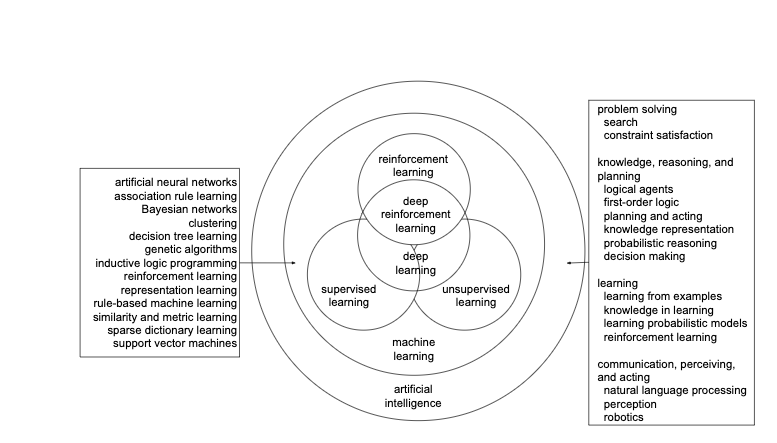
\includegraphics[width=0.5\textwidth]{figures/AI.png}
    \caption{F1 agent follows RL cycle in RL-Studio}
    \label{fig:AI components}
\end{figure}

En este tipo de problemas un agente, como puede ser un coche o un robot, está interactuando en un entorno, como una carretera o un almacén, en cada paso para obtener una recompensa. El agente tiene que aprender cuales son las mejores decisiones y acciones en cada momento para conocer la mejor estrategia a seguir, la politica, que le lleve a optimizar las recompensas en el largo plazo. La recompensa es una de las mas importantes conceptos en RL, debido a que el objetivo buscado es la maximización de los valores esperados de la suma acumulada de una señal. El diseño de la funcion de recompensa en un algoritmo de RL es una mezcla de arte y ciencia, que se consigue a traves de constantes pruebas.

\begin{figure}[ht]
    \centering
    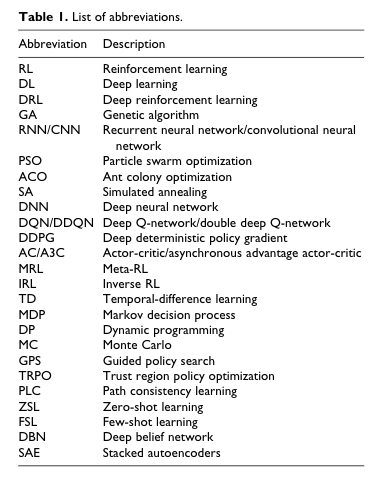
\includegraphics[width=1\textwidth]{figures/list-abbreviations.png}
    \caption{list of abbreviations}
    \label{fig:list_abbreviations}
\end{figure}


En los métodos RL dejamos que el agente encuentre la mejor solución para que pueda generalizarse a problemas similares sin tener que programar explícitamente. Pero ahora, otro tipo de problemas complejos parecen resolverse como una muestra ineficiente producida por el dilema de exploración versus explotación, donde son necesarias millones de iteraciones para encontrar una solución a problemas reales.


\begin{figure}[ht]
    \centering
    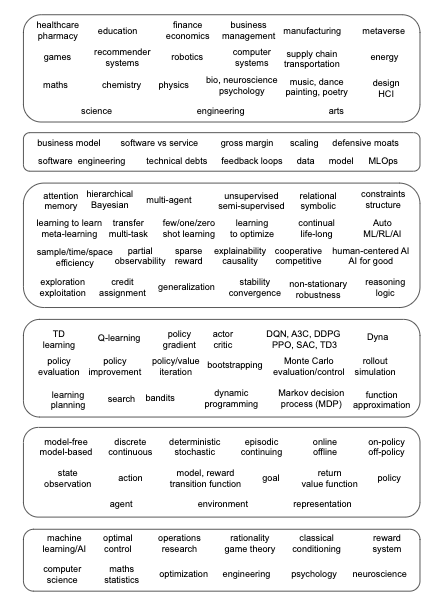
\includegraphics[width=0.7\textwidth]{figures/RL-general.png}
    \caption{General RL frame }
    \label{fig:RL total vision}
\end{figure}


Existen dos taxonomías principales de algoritmos en la RL clásica, \emph{métodos de aprendizaje basados en muestras} o también denominados \textit{algoritmos basados en valores} y \textit{métodos de solución aproximada} o \textit{algoritmos basados en políticas}. El primero se usa en acciones y estados en problemas de baja dimensionalidad y dentro de esta categoría podemos encontrar la programación dinámica, los métodos de Monte-Carlo y los métodos de diferencia temporal. Estos últimos pueden trabajar con escenarios reales con acciones continuas y espacio de estados y la solución que brindan es solo aproximada. Los gradientes de políticas son la familia de métodos más popular \cite{sutton2018reinforcement}.

En escenarios reales, sensores como las cámaras recopilan miles de datos en cada cuadro que deben ser procesados ​​por algoritmos RL. Con la RL clásica eso será intratable. Pero ahora DL con RL nos permite abordar problemas complejos con estados de alta dimensión y acciones continuas, donde RL construye la parte de planificación y DL la parte de aprendizaje de representación. El uso de algoritmos DL dentro del marco RL ha creado el nuevo campo de Deep Reinforcement Learning (DRL).

El desarrollo de modelos RL involucra diferentes pasos. Una es seleccionar el agente con las características y sensores adecuados para leer correctamente la información del entorno. Otra es elegir el algoritmo RL que se adapte al objetivo. Hay docenas dentro de las categorías anteriores y cada una de ellas tiene sus propios parámetros que deben ajustarse. Además, cada simulador tiene características que lo hacen adecuado para un problema específico y, finalmente, el proceso de trabajo requiere pruebas continuas de prueba y error, evaluando los resultados del entrenamiento, ajustando parámetros o incluso cambiando el diseño de ciertos componentes.

\section{Core elements}\label{ch:core}
En esta seccion vamos a mostrar una perspectiva del estado del arte de algoritmos y metodos en RL

%%%%%%%%%%%%%%%%%%%%%%%%%%%%%%%%%%%%%%%%%%%%%%%%%%%%%%%%%%%%%%%%%%%%%%%%%%%%%
\subsection{RL Fundamentals}\label{ss:rl_fundamentals}
Los problemas de RL se pueden modelar como un proceso de decisión de Markov (MDP), que es un marco matemático que se define como una tupla $\left(S, A, P_{a}, R_{a}\right)$, donde $S$ es un conjunto de estados denominado espacio de estado, $A$ es un conjunto de acciones denominado espacio de acción, $P_{a}\left(s, s^{\prime}\right)=\operatorname{Pr}\left (s_{t+1}=s^{\prime} \mid s_{t}=s, a_{t}=a\right)$ es la probabilidad de que la acción $a$ en el estado $s$ en el tiempo $t $ conducirá al estado $s^{\prime}$ en el momento $t+1$ y $R_{a}\left(s, s^{\prime}\right)$ es la recompensa inmediata (o la recompensa inmediata esperada ) recibido después de la transición del estado $s$ al estado $s^{\prime}$, debido a la acción $a$

En cada paso de tiempo discreto $t$, el agente recibe información del entorno, el estado $s_t$, y tiene que realizar una acción $a_t$. Cuando se ejecuta la acción, el entorno envía al agente el siguiente estado $s_{t+1}$ y la recompensa $r$, normalmente un escalar. Una función de política mapea cada estado con la acción. Recuerde que el objetivo principal en RL es maximizar las recompensas, lo que significa aprender la mejor política.
Una idea principal en RL es el concepto de \textit{Función de valor}, que nos dice cómo será la recompensa en el futuro por estar en un estado o por realizar una acción en un estado.
Formalmente, podemos definir una función de valor de un estado $s$ bajo una \textit{política} $\pi$ como \newline

v_{\pi}(s) \doteq \mathbb{E}_{\pi}\left[G_{t} \mid S_{t}=s\right]=\mathbb{E}_{\pi}\ izquierda[\sum_{k=0}^{\infty} \gamma^{k} R_{t+k+1} \mid S_{t}=s\right], \forall s \in \mathcal{S} \newline

Si ponemos la acción dentro de la ecuación anterior. tenemos la \textit{función de valor de acción} para $policy$ $\pi$ como:\newline

$q_{\pi}(s, a) \doteq \mathbb{E}_{\pi}\left[G_{t} \mid S_{t}=s, A_{t}=a\right]=\ mathbb{E}_{\pi}\left[\sum_{k=0}^{\infty} \gamma^{k} R_{t+k+1} \mid S_{t}=s, A_{t }=a\derecho]$\newline

La mayoría de los algoritmos de RL se basan en las dos ecuaciones anteriores.


%%%%%%%%%%%%%%%%%%%%%%%%%%%%%%%%%%%%%%%%%%%%%%%%%%%%%%%%%%%%%%%%%%%%%%%%%%%%%
\subsection{Enfoques RL}\label{ss:rl_enfoques}
Para conocer el valor proporcionado por RL-Studio, es necesario categorizar los puntos principales en el desarrollo de algoritmos RL para generar modelos adecuados para cada dominio específico.

\subsubsection{Model-Free y Model-Based.}\label{ss:models}
En los algoritmos basados en modelos, conocemos el entorno y lo usamos para mejorar el aprendizaje. Por ejemplo, en juegos como el ajedrez o el póquer, las reglas son fijas y los algoritmos de RL las usan para aprender a encontrar mejores soluciones. En los algoritmos sin modelo, aprende políticas que interactúan a través del entorno, tomando las reglas en el proceso. En teoría, este tipo de RL se puede aplicar a cualquier problema.
Pero, de hecho, existen algoritmos que pueden gobernar en un entorno conocido y aprender políticas óptimas. Así que las fronteras están borrosas.

\subsubsection{Agentes en línea y fuera de línea.}\label{ss:onlineoffline}
Cuando un agente aprende directa e inmediatamente del entorno para mejorar su política se llama en línea. En el caso de que el agente aprenda de conjuntos de datos o registros fuera de línea, se llama Fuera de línea.

\subsubsection{En política y fuera de política.}\label{ss:onpolicyoffpolicy}
Con respecto a los agentes que seleccionan una acción definida por su política, los agentes con política aprenden a predecir la recompensa después de seguir la política actual, mientras que los agentes sin política no necesitan seguir ninguna política y pueden aprenderla después de seguir cualquier acción.

\subsubsection{Evaluación de políticas y mejora de políticas.}\label{ss:policyimprov}
La evaluación de políticas o también llamado problema de predicción \cite{sutton2018reinforcement} mejora la estimación de la función de valor. A medida que mejora la estimación, la política se puede mejorar naturalmente eligiendo acciones con avidez en función de la función de valor actualizada. Ambos conceptos unidos en un mismo proceso se denomina \emph{iteración de política generalizada}.


%%%%%%%%%%%%%%%%%%%%%%%%%%%%%%%%%%%%%%%%%%%%%%%%%%%%%%%%%%%%%%%%%%%%%%%%%%%%%
\subsection{Retos y oportunidades de RL}\label{ss:rl_problems}
Es instructivo enfatizar algunos desafíos enfrentados en RL:\\
\begin{itemize}
\item Los algoritmos de RL deben inferir mediante la interacción de prueba y error con el entorno y la única señal de aprendizaje que recibe el agente es la recompensa. Cuando el entorno no muestra ninguna recompensa hasta alcanzar la meta, los agentes navegan por el mundo sin retroalimentación y se enfrenta a \emph{recompensas escasas}.
\item El agente realiza una acción que conduce a una observación en muchos pasos de tiempo que pueden contener \textit{correlaciones temporales fuertes}.
\item \textit{El problema de la asignación (temporal) del crédito} cuando las consecuencias de las acciones se obtienen a largo plazo.
\item Eficiencia de muestreo
\item exploracion vs explotacion
\item (TOMADO DE Deep Rl opportunities and challenges - Yuxi Li) La reproducibilidad es un problema para la RL profunda, es decir, los resultados experimentales están influenciados por hiperparámetros, incluida la arquitectura de la red y la escala de recompensa, las semillas y los ensayos aleatorios, los entornos y las bases de código.(Reproducibility is an issue for deep RL, i.e., experimental results are influenced by hyperparameters, including network architecture and reward scale, random seeds and trials, environments, and codebases (Henderson et al.,2018))
\item Los enfoques de función de valor con aproximación de función, en particular con DNN, se encuentran con la tríada mortal, es decir, inestabilidad y/o divergencia causada por la integración de fuera de política, aproximación de función y bootstrapping.

\item La especificación de la recompensa puede causar problemas y una función de recompensa puede no representar la intención del diseñador.

\item Dulac-Arnold et al. (2021) identifican nueve desafíos para que RL se implemente en escenarios de la vida real, a saber,
\begin{itemize}
    \item aprender sobre el sistema real a partir de muestras limitadas
    \item retrasos del sistema
    \item estados de alta dimensión y espacios de acción
    \item satisfacer las restricciones del entorno
    \item observabilidad parcial y no estacionariedad
    \item funciones de recompensa con múltiples objetivos o mal especificadas
    \item inferencia en tiempo real
    \item entrenamiento de RL fuera de línea a partir de registros fijos
    \item políticas explicables e interpretables
    
\end{itemize}


\end{itemize}


[TOMADO de Robotics 2013, 2, 122-148; doi:10.3390/robotics2030122, Reinforcement Learning in Robotics: Applications and Real-World Challenges 2013]
However, creating a good policy representation is not a trivial problem, due to a number of serious challenges posed by the high requirements from a robotic system, such as:

\begin{itemize}   
    \item suavidad: la representación de políticas debe codificar trayectorias suaves y continuas, sin aceleraciones ni tirones repentinos, para que sea seguro para el propio robot y también para reducir su consumo de energía;
    \item seguridad: la política debe ser segura, no solo para el robot (en términos de límites de articulación, límites de torsión, restricciones del espacio de trabajo, obstáculos, etc.), sino también para las personas que lo rodean;
    \item exploración gradual: la representación debe permitir una exploración gradual e incremental, de modo que la política no cambie mucho repentinamente; por ejemplo, en políticas basadas en acciones de estado, cambiar la acción de la política en un solo estado podría causar un cambio repentino y dramático en el comportamiento general del sistema al seguir esta nueva rama de la política, lo cual no es deseable ni para el robot, ni para las personas que lo rodean. Sin embargo, en algunos casos, puede ser necesario un cambio de paso considerable, por ejemplo, una tarea de navegación en la que un robot necesita decidir si ir a la izquierda o a la derecha para evitar un obstáculo;
    \item escalabilidad: para poder escalar a grandes dimensiones y para tareas más complejas; por ejemplo, un robot humanoide típico hoy en día tiene muy por encima de 50 DoF;
    \item compacidad: a pesar del alto DoF de los robots, la política debe usar una codificación muy compacta, por ejemplo, es imposible usar directamente todos los puntos en una trayectoria como parámetros de política;
    \item adaptabilidad: la parametrización de la política debe ser adaptable a la complejidad y fidelidad de la tarea, por ejemplo, levantamiento de pesas versus microcirugía;
    \item resolución múltiple: diferentes partes de la parametrización de la política deben permitir una resolución/precisión diferente;
    \item imparcialidad: la parametrización de políticas debe funcionar sin conocimiento previo sobre la solución que se busca y sin restringir innecesariamente el alcance de la búsqueda de posibles soluciones;
    \item anterior/sesgo: siempre que sea factible, debería ser posible agregar información previa (también llamada sesgo) para impulsar los enfoques de búsqueda de políticas,
    \item regularización: la política debe permitir incorporar la regularización para guiar la exploración hacia tipos deseados de políticas;
    \item tiempo-independencia: esta es la propiedad de una política de no depender del tiempo o la posición precisos, para hacer frente a perturbaciones imprevistas;
    \item embodiment-agnóstico: la representación no debe depender de ninguna encarnación particular del robot, por ejemplo, las políticas basadas en trayectorias conjuntas no se pueden transferir fácilmente a otro robot;
    \item invariance: la política debe ser una representación invariable de la tarea (p. ej., rotación invariable, escala-invariante, posición-invariante, etc.);
    \item correlaciones: la política debe encapsular las correlaciones entre las variables de control (por ejemplo, señales de control del actuador), similares a las sinergias motoras que se encuentran en los animales;
    \item globality: la representación debería ayudar al algoritmo RL a evitar los mínimos locales;
     \item periodicity: para poder representar fácilmente movimientos periódicos/cíclicos, que ocurren a menudo en robótica (p. ej., para locomoción, diferentes modos de andar, para manipulación, limpieza,  movimientos, etc.);
    \item analizabilidad: facilidad para visualizar y analizar la política (por ejemplo, probar su estabilidad por polos) análisis, etc.);
        \item multidimensionalidad: para poder usar de manera eficiente retroalimentación de alta dimensión sin la necesidad de convertirlo en un valor escalar utilizando una suma ponderada de componentes;
    \item convergencia: para ayudar al algoritmo RL a converger más rápido a los óptimos (posiblemente locales).

       
\end{itemize}

Aqui encontramos una lista de Temas Candentes en RL

\begin{itemize}
    \item end-to-end  or  not
    \item auxiliary  or  un/self-supervised  reward
    \item prior  knowledge
    \item meta-learning
    \item hierarchical
    \item multi-agent
    \item causal
    \item symbolic
    \item relational
    \item explainable
    \item safety
    \item robustness
    \item AI for good
\end{itemize} 



%%%%%%%%%%%%%%%%%%%%%%%%%%%%%%%%%%%%%%%%%%%%%%%%%%%%%%%%%%%%%%%%%%%%%%%%%%%%%
\subsection{Algoritmos RL}\label{ss:rl_algorithms}

\begin{figure}[ht]
    \centering
    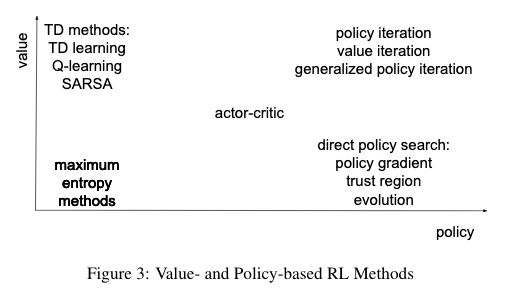
\includegraphics[width=1\textwidth]{figures/algorithms-RL.png}
    \caption{Algoritmos de RL}
    \label{fig:algorithmsRL}
\end{figure}


\subsubsection{Métodos de aprendizaje basado en muestras o valor de acción.}\label{ss:samplebased}
En esta categoría podemos encontrar métodos de \emph{programación dinámica} (DP) que funcionan en un modelo perfecto del entorno como un MDP. Satisfacen las ecuaciones de optimalidad de Bellman. \emph{Monte Carlo} son otros métodos que utilizan sólo la experiencia. Básicamente, trabajan con retornos de muestra promedio, recolectando todas las recompensas en cada paso de los episodios. Aquí podemos encontrar el Monte Carlo Tree Search (MCTS) utilizado en el programa de AlphaGo \cite{silver2016mastering}. Aprendizaje de \emph{diferencia temporal} (TD) que es una combinación de los dos métodos anteriores. Aquí podemos encontrar el algoritmo \emph{SARSA} \cite{rummery1994line} que es un control TD dentro de la política y \emph{Q-learning} \cite{watkins1989learning}, quizás el algoritmo RL más conocido, un fuera de la política Algoritmo de control TD. Algunos algoritmos DRL caen en esta categoría, como \emph{Deep Q-Network} (DQN) que se usó para el éxito en los juegos Atari 2600\cite{mnih2015human}

\begin{itemize}
    \item Deep Q-learning
    \item Double DQN
    \item Prioritized experience replay
    \item dueling architecture
    \item rainbow
    \item retrace
\end{itemize}
Dentro de esta categoria podemos encontrar la funcion de valor distribucional y funcion de valor general (aqui tenemos HORCE, aproximadores de funcion de valor universales y Hindsight experience replay ) (Li Y. 2018)



\subsubsection{Métodos basados en políticas.}\label{ss:policybased}
A diferencia de los métodos anteriores, estos otros buscan políticas $\pi_{\phi}$, normalmente realizando un ascenso de gradiente $J\left(\pi_{\phi}\right)=J(\phi)$ con respecto a la política parámetros $\phi$. \emph{Los Métodos Actor-Crítico} son una versión TD del Gradiente de Política. Tienen una red, el \emph{Actor}, que decide qué acción se debe tomar en función del enfoque de gradiente de políticas. Y la otra red, la \emph{crítica}, informa al actor qué tan buena fue la acción tomada y cómo debe ajustarse, según la función de valor de cálculo. Las técnicas de DL se utilizan ampliamente para aproximar los parámetros de las políticas, por lo que se han desarrollado muchos algoritmos de DRL en esta categoría, como PPO \cite{schulman2017proximal} o DDPG\cite{lillicrap2015continuous}.

Una division mas detallada es:

\begin{itemize}
    \item Policy gradient
    \item Actor-critic
    \item metodos de region de confianza TRPO, PPO
    \item policy gradient con aprendizaje fuera de politica: soft Q-learning, path consistency learning, 
    
\end{itemize}

%%%%%%%%%%%%%%%%%%%%%%%%%%%%%%%%%%%%%%%%%%%%%%%%%%%%%%%%%%%%%
\section{rewards??}

%%%%%%%%%%%%%%%%%%%%%%%%%%%%%%%%%%%%%%%%%%%%%%%%%%%%%%%%%%%%%
\section{Representación}
El aprendizaje de representacion es un enfoque para encontrar automaticamente buenas caracteristicas de cualquier punto en la cadena de RL, por ejemplo a la representacion del problema como un MDO o POMDP o PSR (predictive state representation)
\subsubsection{Aproximaciones clasicas:}
\begin{itemize}
    \item Aproximacion de funcion: tile coding, RBFs
    \item Metodos para resolver MDP y POMDP
    \item Distribucion de estado y de accion-estado
\end{itemize}

\subsubsection{Redes Neuronales:}
\begin{itemize}
    \item Aprendizaje de representacion: smoothness, linearity, multiple explanatory factors, causal factors, hierarchical organization of explanatory factors, Shared factors across tasks, manifolds, Natural clustering, temporal and spatial coherence, sparsity, simplicity of factor dependencies
    \item arquitecturas de Redes neuronales: CNN, RNN, MLN y las nuevas especificas para RL: VIN, predictron, VPN, IA2, TreeQN, ATreeC, TDM, MCT
\end{itemize}

\subsubsection{Conocimiento y razonamiento:}
\begin{itemize}
    \item funcion de valor general GVF, 
    \item hierarchical RL, 
    \item RL relacional, 
    \item casualidad, 
    \item razonamiento, inteligencia humana
\end{itemize}
    
%%%%%%%%%%%%%%%%%%%%%%%%%%%%%%%%%%%%%%%%%%%%%%%%%%%%%%%%%%%%%
\section{Important mechanisms}\label{ch:important_mechanisms}
[PUNTO 4.5 ]
Li and Malik (2017),  along with a blog,14divide various learning to learn methods into three categories:  learning what to learn; learning which model to learn;  and  learning  how  to  learn

\subsection{Learning to learn}, a.k.a.  meta-learning, is learning about some aspects of learning.   It  includes  concepts  as  broad  as  transfer  learning,  multi-task  learning,one/few/zero-shot  learning,  learning  to  reinforcement  learn,  learning  to  optimize,  learning  combinatorial  optimization,  hyper-parameter  learning,  neuralarchitecture design, automated machine learning (AutoML)/AutoRL/AutoAI
Transfer Learning: sim2real

\subsection{Multi-Agent RL} es la integracion de sistemas multiagentes. Permite modelar las interacciones entre agentes.

\subsection{Hierarchical RL} se usa en temas de recompensas sparse y/o largos horizontes con la exploración en el espacio de los objetivos de alto nivel. La estructura modular de los enfoques jerárquicos de RL por lo general favorece la transferencia y el aprendizaje de múltiples tareas. Los conceptos de subobjetivo, opción, habilidad y macroacción están relacionados. El RL jerárquico sigue el principio general de diseño de algoritmos de divide y vencerás, de modo que los objetivos difíciles, p. aquellos con escasas recompensas a largo plazo se reemplazan con objetivos secundarios fáciles, p. aquellos con recompensas densas a corto plazo, y los algoritmos RL, por ejemplo, basados en políticas o basados en valores, combinados con representaciones, se utilizan para resolver subobjetivos fáciles y, finalmente, para lograr objetivos difíciles.

\subsection{explainable RL}


\subsection{Attention and memory}
La atención es un mecanismo para enfocarse en las partes sobresalientes. La memoria proporciona almacenamiento de datos a largo plazo. La atención puede ser un enfoque para el direccionamiento de la memoria.

\subsection{Unsupervised learning}
Los entornos pueden contener abundantes señales de entrenamiento posibles, que pueden ayudar a acelerar el logro del objetivo principal de maximizar las recompensas acumulativas, por ejemplo, los cambios de píxeles pueden implicar eventos importantes, y las tareas de recompensa auxiliar pueden ayudar a lograr una buena representación de los estados de recompensa. Esto puede ser incluso útil cuando las recompensas extrínsecas rara vez se observan.

\begin{itemize}
    \item aprendizaje auxiliar no supervisado
    \item redes adversarias generativas
    \item redes de consulta generativas
    \item jugando viendo youtube
    
    
\end{itemize}

\subsection{Relational RL}


%%%%%%%%%%%%%%%%%%%%%%%%%%%%%%%%%%%%%%%%%%%%%%%%%%%%%%%%%%%%%
\section{Aplicaciones}\label{ch:aplicaciones}

\begin{figure}[ht]
    \centering
    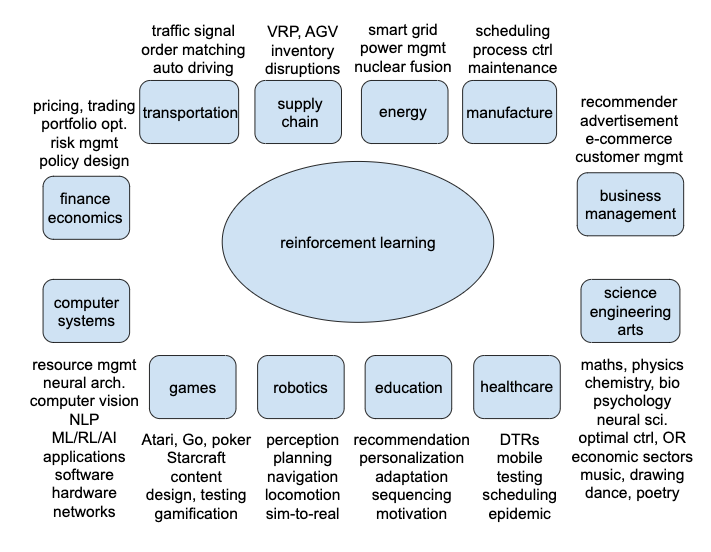
\includegraphics[width=1\textwidth]{figures/RL-apps.png}
    \caption{Applications}
    \label{fig:RL applicability}
\end{figure}


\subsubsection{Robótica.}\label{ss:robotica}

\begin{figure}[ht]
    \centering
    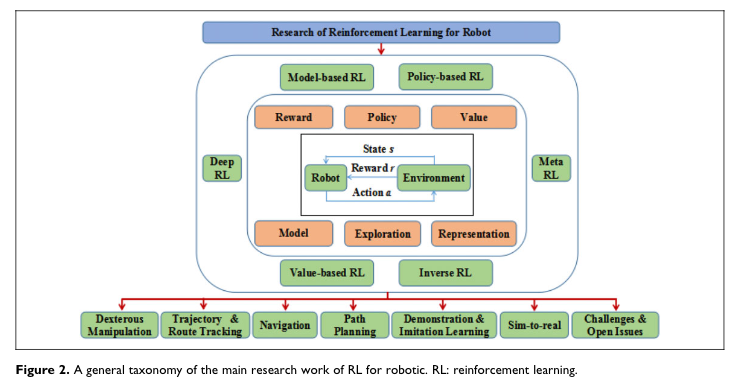
\includegraphics[width=1\textwidth]{figures/researchwork_robotics.png}
    \caption{research works}
    \label{fig:robotics_research}
\end{figure}


\subsubsection{Vehiculos autonomos.}\label{ss:vehi_auton}



%%%%%%%%%%%%%%%%%%%%%%%%%%%%%%%%%%%%%%%%%%%%%%%%%%%%%%%%%%%%%
\bibliography{thesis.bib}% common bib file
%\bibliographystyle{IEEEtran}
\bibliographystyle{spmpsci}

\end{document}